\chapter{ESTUDO DE CASO}

Este capítulo apresenta um estudo de caso com a implantação de um ambiente de Integração Contínua no projeto da Biblioteca Digital da Rede Nacional de Pesquisa e Inovação (RENAPI). Este estudo de caso foi idealizado devido ao fato do processo de Integração Contínua realizado no Núcleo de Pesquisa em Sistema de Informação (NSI) do IFF-Campos apresentar problemas, junto com o ideal de melhorar a prática de integração no grupo.

\section{Ambiente estudado}

O estudo de caso deste trabalho foi realizado no NSI. O NSI surgiu em abril de 2002 e desde essa época vem utilizando e estimulando o uso de tecnologias de software livres.

Durante a fase de criação deste estudo de caso, o núcleo contava com 32 bolsistas, subdivididos entre vários projetos. Dois destes projetos estavam diretamente relacionados com este trabalho: o projeto da Biblioteca Digital da RENAPI e o Quali-Ágil.

O portal da Biblioteca Digital da RENAPI visa disponibilizar um acervo bibliográfico digital de maneira a contribuir para a disseminação do material científico e tecnológico produzido na rede de Instituições de Educação Profissional Científica e Tecnológica (EPCT) - como artigos, monografias, dissertações, teses e periódicos, promovendo a disseminação nacional e internacional deste conteúdo, visando colaborar na qualificação do material humano da rede e na disseminação de conhecimento.

O Quali-Ágil é um projeto, que visa o estudo e desenvolvimento de ferramentas e metodologias para aumentar a qualidade de projetos de software que usam metodologias ágeis.

A Biblioteca Digital é um dos projetos mais importantes do NSI. Por tal motivo, ele precisa ser estável e confiável, devido a seu grande porte e visibilidade. Para alcançar tais objetivos, a Integração Contínua é uma boa prática. O papel do Quali-Ágil neste trabalho foi ajudar no gerenciamento e implantação do ambiente de Integração Contínua.

\section{Situação anterior}

O NSI não tinha um processo de Integração Contínua consistente. O processo era feito da seguinte maneira: O Buildbot, servidor de Integrção Contínua utilizado pelo NSI, não tinha o papel característico dos servidores de integração, cuja tarefa é fiscalizar o repositório à procura de mudanças. O Buildbot ficou responsável por executar o \textit{script} de \textit{build} em um determinado horário todos os dias, caracterizando o mecanismo de \textit{build} programado. Da forma como era feita a integração no NSI, o modelo de integração utilizado era o Assíncrono.

O \textit{script} de \textit{build} criado utilizava o Buildout\footnote{http://www.buildout.org/}, sendo esta uma ferramenta \textit{open source} de construção de software criada em Python\footnote{http://www.python.org/}, fornecendo suporte à criação de aplicações.

Quando chegava a hora do \textit{build} ser executado, ele compilava todo o sistema e executava a suíte de testes. Caso algum teste falhasse, a equipe de desenvolvimento recebia um e-mail, sendo este o mecanismo de \textit{feedback} escolhido, com a notificação da falha do \textit{build}.

\section{Problemas}

Uma recomendação para ambientes que usam a Integração Contínua é sempre manter a base de dados estável. Por indisciplina da equipe esta recomendação não era atendida já que, toda vez que algum teste não passava, a equipe recebia a notificação pelo e-mail e mesmo assim o código do repositório ficava inconsistente por muito tempo. A medida correta a ser tomada era corrigir o erro o quanto antes, entretanto o que acontecia era a persistência do erro por dias, ou até mesmo, meses.

Ademais, como a execução do \textit{build} acontecia somente à noite, caso o mesmo viesse a falhar, a tarefa de descobrir a localização do erro era mais difícil. Muitos \textit{commits} eram realizados no período da tarde, todavia nenhum deles ativava o \textit{script} de \textit{build}. Dessa forma, quando o \textit{build} quebrava, era mais difícil saber qual \textit{commit} fez o \textit{build} falhar, visto que foram realizados vários envios de código naquele determinado dia.

O \textit{feedback} da integração não era instantâneo, já que o \textit{build} era programado e só era executado em determinado horário do dia. Logo, para o desenvolvedor saber se a alteração que ele enviou para o repositório foi integrada corretamente, ele precisava esperar até o outro dia para saber o resultado da integração.

Além disso, a idéia do botão da integração não era completa, pois não se conseguia ter software funcional com apenas o clique de um botão. De acordo com o princípio do botão da integração, com apenas um comando deve ser gerado software funcional. Para se obter o software final era necessário a realização de uma série de etapas manuais, o que não condiz com a idéia do botão da integração.

\section{Proposta para implantação da Integração Contínua}

Como a Biblioteca Digital é um projeto de grande porte que está em andamento, decidiu-se por utilizar o modelo de Integração Contínua Assíncrona por este ser de mais rápida implantação e adaptação, comparado com o modelo de integração Síncrono.

O processo começava com os desenvolvedores obtendo o código do repositório da RENAPI para realizar as alterações. Após modificar o código fonte, os desenvolvedores executavam a suíte de testes à procura de falhas. Obviamente, se alguma falha fosse encontrada, eles teriam que corrigí-la. Caso contrário, eles enviariam o código alterado para o repositório da RENAPI.
Nesse estágio, havia uma máquina de integração que possuia um servidor de Integração Contínua, o Hudson. Ele tinha como responsabilidade fiscalizar o repositório da RENAPI constantemente à procura de qualquer modificação no código fonte do projeto. Caso o Hudson encontrasse alguma alteração no repositório, ele iria resgatar e executar o \textit{script} de \textit{build} na máquina de integração. Toda suíte de testes era executada e, se alguma falha acontecesse, o \textit{build} falharia e a equipe de desenvolvimento receberia um e-mail avisando acerca da falha.

O ambiente de Integração Contínua realizado no projeto pode ser visto na Figura \ref{componentes_estudo}

\begin{figure}[ht]
    \centering
    \scalebox{0.7}{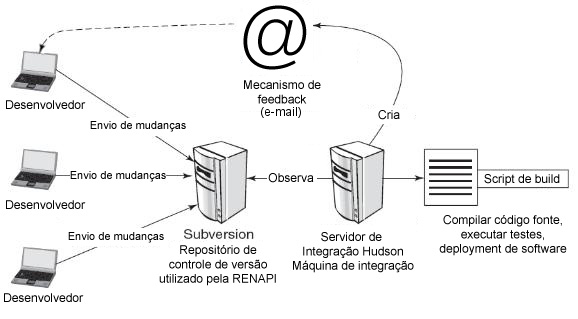
\includegraphics{figuras/componentes_estudo}}
    \caption{Componentes do ambiente de Integração Contínua do estudo de caso.}
    \label{componentes_estudo}
\end{figure}

\section{Como foi feita a implantação}

Para a implantação foi alocada um máquina com processador Pentium 4, 2 GB de Memória RAM e 80 GB de HD. Nesta máquina foi instalado o sistema operacional Debian 5, o mesmo utilizado pelo sistema em produção.

A máquina de integração era totalmente virgem, ou seja, só foi instalado o Debian 5, o Hudson versão 1.357, bem como o Java que é dependência do servidor Hudson. Para instalar o Hudson foi necessário adicionar a chave do repositório Hudson ao sistema com os comandos apresentados na Figura \ref{comandos_chave}.

\begin{figure}[ht]
    \centering
    \scalebox{0.7}{
\includegraphics{figuras/comandos_chave}}
    \caption{Comandos para adicionar chave do repositório Hudson}
    \label{comandos_chave}
\end{figure}

Após isto, bastou somente instalar o Hudson através dos seguintes comandos, como mostra a Figura \ref{comandos_hudson}:

\begin{figure}[ht]
    \centering
    \scalebox{0.7}{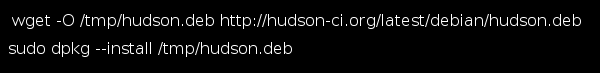
\includegraphics{figuras/comandos_hudson}}
    \caption{Comandos para instalar o Hudson}
    \label{comandos_hudson}
\end{figure}

Instalando o Hudson dessa forma, ele pode ser atualizado pelo gerenciador de pacote do Debian, o apt-get, o que viabiliza o uso da última versão deste servidor de Integração Contínua.

Devidamente instalado, o Hudson foi acessado pela porta 8080, atráves do endereço \textit{http://localhost:8080}. A tela principal do Hudson, pode ser vista na Figura \ref{hudson_principal}

\begin{figure}[ht]
    \centering
    \scalebox{0.6}{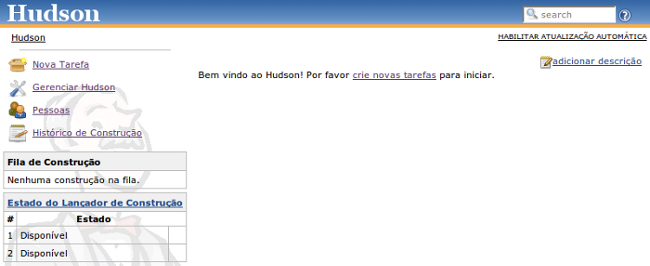
\includegraphics{figuras/hudson_principal}}
    \caption{Tela principal do Hudson}
    \label{hudson_principal}
\end{figure}

O primeiro passo foi fazer a configuração da notificação de e-mail. Caso houvesse alguma falha no \textit{build}, a equipe de desenvolvedores deveria receber um e-mail de notificação da quebra do \textit{build}. Para configurar tal notificação acessou-se o \textit{link} ``Gerenciar Hudson'' na tela principal do Hudson e logo após o ítem ``Configurar Sistema''.

Na seção ``Notificação de E-mail'' o campo ``Servidor SMTP'' foi preenchido com o respectivo servidor de SMTP e o campo ``Endereço de E-mail do Administrador do Sistema'' foi preenchido com o e-mail do responsável pela administração do Hudson. A seção ``Notificação de E-mail'' é demonstrada na Figura \ref{notificacao_email}.

\begin{figure}[ht]
    \centering
    \scalebox{0.7}{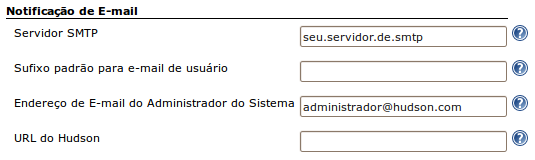
\includegraphics{figuras/notificacao_email}}
    \caption{Tela de configuração da Notificação de E-mail no Hudson}
    \label{notificacao_email}
\end{figure}

Feita a configuração da notificação de e-mail, foi instalado o \textit{plugin} do Selenium\footnote{http://seleniumhq.org/}, que é um \textit{framework} para automatização de testes para aplicações \textit{Web}, sendo este usado nos testes de aceitação do projeto da Biblioteca Digital. Para instalar este \textit{plugin} acessou-se o link ``Gerenciar Hudson'' na tela principal do Hudson e logo após o ítem ``Gerenciar Plugins''. Em seguida foi acessada a aba ``Disponíveis''. Nesta aba, aparecem todos os \textit{plugins} que o Hudson oferece para instalação. Na seção ``Cluster Manegement and Distributed Build (Gerenciamento de \textit{Cluster} e \textit{Build} Distribuído)'' instalou-se o ``Selenium Plugin'', que é responsável por inicializar este \textit{framework}. A instalação do ``Selenium Plugin'' pode ser vista na Figura \ref{selenium_plugin}

\begin{figure}[ht]
    \centering
    \scalebox{0.65}{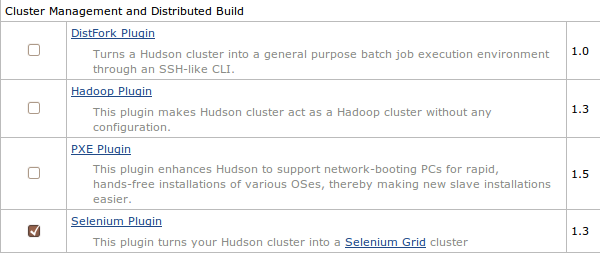
\includegraphics{figuras/selenium_plugin}}
    \caption{Tela de instalação do ``Selenium Plugin'' no Hudson}
    \label{selenium_plugin}
\end{figure}

Após a instalação desse \textit{plugin}, acessou-se no menu lateral esquerdo da tela principal o ítem ``Gerenciar Hudson'', sucedido do ítem ``Manage Nodes (Gerenciamento de Nós)'', que apresenta uma tela de configuração e criação de novos nós. No menu lateral esquerdo, há o ítem ``New Node (Novo Nó)'' que representa a criação de um novo nó. Clicou-se nele e na tela posterior foi preenchido o campo ``Node name (Nome do Nó)'' com o conteúdo ``Selenium Grid'' e selecionado a opção ``Dumb Slave'', como mostra a Figura \ref{hudson_novo_no}.

\begin{figure}[ht]
    \centering
    \scalebox{0.7}{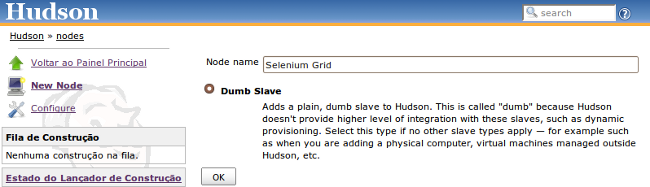
\includegraphics{figuras/hudson_novo_no}}
    \caption{Tela de criação de nós no Hudson}
    \label{hudson_novo_no}
\end{figure}

Na tela seguinte foi nescessário configurar o números de processos concorrentes no processador, para isso foi preenchido o campo ``Número de executores'' com o valor ``10'', ou seja, será permitido 10 processos concorrentes do Selenium no processador. Após isso, o campo ``Diretório de trabalho do sistema remoto'' foi preenchido com o caminho do diretório onde o Hudson deposita seus arquivos de configuração. Em ``Uso'' selecionou-se a opção ``Leave this machine for tied jobs only (Deixar esta máquina somente para trabalhos amarrados)'', o que significa que o nó somente será utilizado quando este for configurado por uma determindada tarefa, permanecendo os demais campos com o valor padrão. Esta configuração pode ser observada na Figura \ref{configuracao_no}.

\begin{figure}[ht]
    \centering
    \scalebox{0.6}{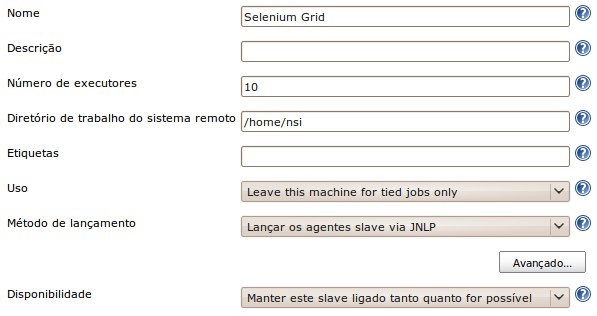
\includegraphics{figuras/configuracao_no}}
    \caption{Tela de configuração de nós no Hudson}
    \label{configuracao_no}
\end{figure}

O próximo passo foi iniciar o nó recém criado, Selenium Grid. Para isso foi pressionado o botão ``Launch (Iniciar)'', e salvo o arquivo ``slave-agent.jnlp'' no mesmo diretório configurado no campo ``Diretório de trabalho do sistema remoto''. Após isso, foi colocado no arquivo /etc/rc.local a linha de comando ``javaws /home/nsi/slave-agent.jnlp'', linha esta que faz com que o Selenium Grid seja inicializado automaticamente, evitando a inicialização manual toda vez que a máquina for ligada.

Depois da configuração do Selenium, acessou-se o link ``Nova Tarefa'' no menu lateral esquerdo da tela principal. Nesta tela, colocou-se o nome da tarefa como ``Biblioteca Digital'' e escolheu-se a opção ``Construir um projeto de software free-style'', como mostra a Figura \ref{hudson_nova_tarefa}.

\begin{figure}[ht]
    \centering
    \scalebox{0.7}{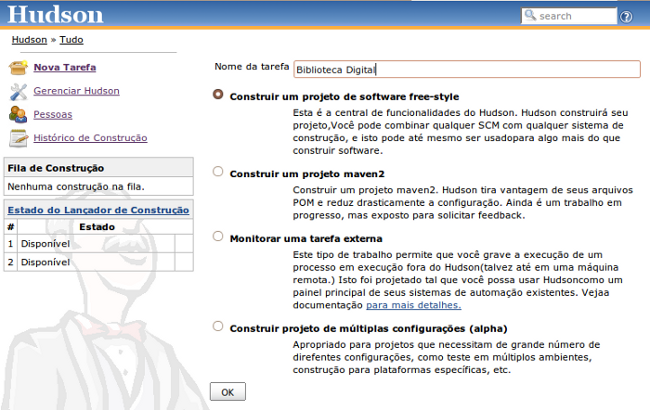
\includegraphics{figuras/hudson_nova_tarefa}}
    \caption{Tela de criação de tarefas no Hudson}
    \label{hudson_nova_tarefa}
\end{figure}

Após preencher os dados requisitados, clicou-se em ``OK'' e uma nova tela foi aberta com dados para configuração da nova tarefa. Na opção ``Tie this project to a node (Amarrar este projeto a um nó)'' escolheu-se o nó criado anteriormente, no caso o Selenium Grid, como demonstra a Figura \ref{configuracao_tarefa_selenium}.

\begin{figure}[ht]
    \centering
    \scalebox{0.7}{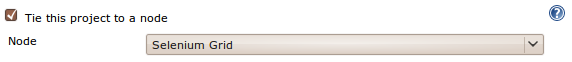
\includegraphics{figuras/configuracao_tarefa_selenium}}
    \caption{Tela de uma tarefa sendo ligada ao Selenium}
    \label{configuracao_tarefa_selenium}
\end{figure}

O próximo passo foi configurar o Sistema de Controle de Versão utilizado pelo projeto da Biblioteca Digital, o Subversion. Na seção ``Gerenciamento de Código Fonte'' foi selecionado a opção ``Subversion'', preencheu-se o campo ``URL do projeto'' com o endereço onde se encontra o repositório da Biblioteca Digital. A opção ``Usar atualização'' foi marcada, para que a cada \textit{build} os arquivos do repostório sejam atualizados automaticamente. A Figura \ref{configuracao_tarefa_subversion} demostra este processo de configuração do Subversion.

\begin{figure}[ht]
    \centering
    \scalebox{0.7}{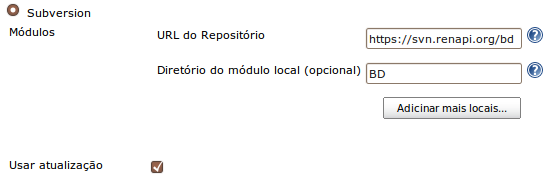
\includegraphics{figuras/configuracao_tarefa_subversion}}
    \caption{Tela de configuração do Subversion em uma tarefa}
    \label{configuracao_tarefa_subversion}
\end{figure}

Na seção ``Disparadores de Construção'' foi marcada a opção ``Consultar periodicamente o SCM''. O campo ``Agenda'' que apareceu, foi preenchido com ``0,30 * * * *'', que segue o padrão Cron, o que significa que o Hudson fiscalizava o repositório no minuto ``0'' e ``30'' de cada hora, todos dias do mês, todos meses e todos dias da semana. Se alguma mudança acontecesse no repositório em alguma dessas fiscalizações, o \textit{build} era disparado. Essa configuração é visualizada na Figura \ref{configuracao_tarefa_consulta}.

\begin{figure}[ht]
    \centering
    \scalebox{0.7}{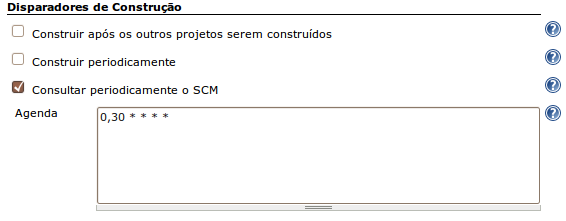
\includegraphics{figuras/configuracao_tarefa_consulta}}
    \caption{Tela de configuração de fiscalização de repositório em um tarefa}
    \label{configuracao_tarefa_consulta}
\end{figure}

Na seção ``Construção'' foi escolhida a opção ``Add Build Step (Adicionar etapa de \textit{build})'' e depois a opção ``Executar shell''. A respectiva caixa da opção ``Executar shell'' foi preenchida com os comandos referentes ao \textit{build}. A Figura \ref{configuracao_tarefa_build} exibe esta etapa.

Por último, na seção ``Ações pós-contrução'', marcou-se a opção ``Notificação de E-mail'' e no campo ``Destinatários'' colocou-se o endereço de e-mail de todos os desenvolvedores da equipe de desenvolvimento da Biblioteca Digital. A Figura \ref{configuracao_tarefa_email} demonstra como fazer esta configuração.

\begin{figure}[ht]
    \centering
    \scalebox{0.7}{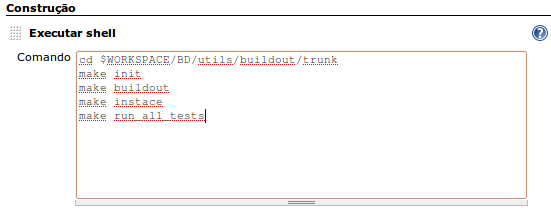
\includegraphics{figuras/configuracao_tarefa_build}}
    \caption{Tela com comandos de execução de um \textit{build} em uma tarefa}
    \label{configuracao_tarefa_build}
\end{figure}

Portanto, esta tarefa foi configurada para obter os arquivos do repositório, executar o \textit{script} de \textit{build}, executar testes e enviar e-mail em caso de quebra do \textit{build}.

\begin{figure}[ht]
    \centering
    \scalebox{0.7}{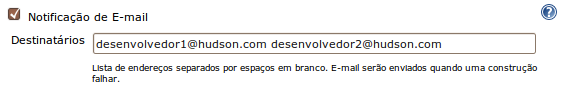
\includegraphics{figuras/configuracao_tarefa_email}}
    \caption{Tela com configuração de envio de e-mail em uma tarefa}
    \label{configuracao_tarefa_email}
\end{figure}

\section{Dificuldades para a implantação}

Uma dificuldade encontrada foi com o \textit{script} de \textit{build}. Para configurar todo o sistema no \textit{script}, foi necessário um esforço maior do que o esperado. O \textit{script} apresentou problemas que exigiram bastante dos desenvolvedores, como por exemplo alguns trechos de código que estavam estáticos, assim dificultando a dinamização do \textit{build}.

Além disso, como o NSI possui muitos desenvolvedores e pesquisadores, alocar a máquina de integração tornou-se uma tarefa difícil. Como a máquina de integração era um computador pessoal (\textit{desktop}), ela ocupava o espaço que um desenvolvedor ocuparia. Aliado a isto, como a máquina deve ser usada exclusivamente para a integração do sistema, nenhuma pessoa deveria fazer uso da máquina.

Outra dificuldade que tomou bastante tempo foi o fato dos testes do projeto estarem falhando. Como o \textit{script} de \textit{build} executava todos os testes do sistema, foram descobertos alguns erros. Logo, como deve-se sempre manter o repositório consistente, alguns dias foram necessários para consertar os erros, inclusive para que o processo começasse de forma correta.

\section{Resultados obtidos}

No estudos de caso desse trabalho foi utilizado um Sistema de Controle de Versão chamado Subversion, que se encontra no endereço https://svn.renapi.org/bd.

O repositório de código era monitorado, e caso alguma mudança fosse detectada, o \textit{script} de \textit{build} era executado, realizando a instalação dos módulos, a execução dos testes, bem como o \textit{deployment} do sistema.

O \textit{build} é auto-testável, ou seja, fazia com que toda a integração do sistema fosse mais facilmente testada.

Uma máquina de integração foi alocada exclusivamente para o processo de integração. Ela não foi utilizada por nenhum desenvolvedor da equipe e continha somente os requisitos necessários para a integração do sistema.

\section{Problemas remanescentes}

A execução dos testes de cada módulo do sistema fez com que testes unitários e de aceitação fossem executados juntos. Com isso, inúmeras inicializações do Selenium eram feitas para execução dos testes de aceitação de cada módulo, acarretando em um tempo maior de \textit{build}. Essas inicializações ocorriam pelo fato do processo do Selenium ser inicializado e finalizado para cada módulo, ou seja, um único processo não poderia ser aproveitado pelos demais módulos. Logo, esse transtorno do Selenium e a alta complexidade do projeto, fizeram com que a integração de apenas cinco módulos estivesse em torno de quarenta minutos.

O sistema inteiro ainda não estava sendo integrado completamente. Somente uma parte do projeto estava inserida no processo de Integração Contínua. Isso ocorria porque integrar todo o sistema iria aumentar exageradamente o tempo de execução do \textit{build}.

O Hudson, que estava sendo executado na máquina de integração, não podia ser visto pelos desenvolvedores da equipe que estivessem fora do IFF. O ideal era que de qualquer lugar, qualquer pessoa pudesse ver como estava a situação do \textit{build} naquele momento.
